% \chapter{Implementation}
\chapter{Hiện thực}
\label{ch:implementation}

\section{Giao diện người dùng}
\label{sec:frontend_implementation}

\begin{figure}
    \centering
    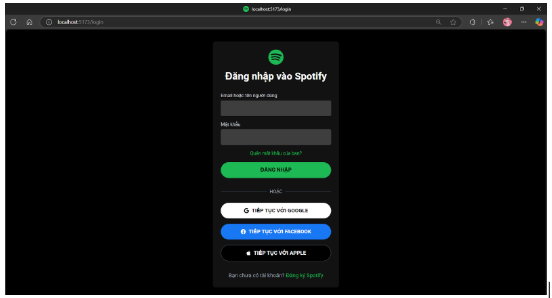
\includegraphics[width=1\linewidth]{images/ui-login.png}
    \caption{Giao diện đăng nhập}
    \label{fig:ui-login}
\end{figure}

\begin{figure}
    \centering
    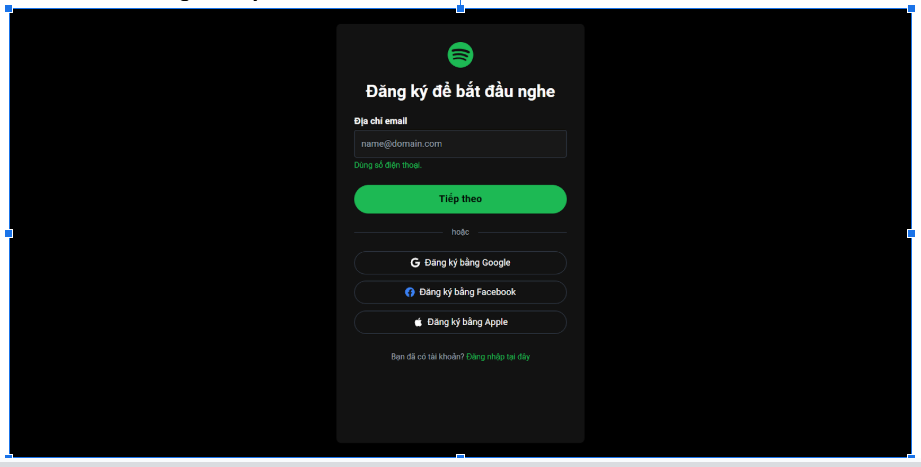
\includegraphics[width=1\linewidth]{images/ui-signup.png}
    \caption{Giao diện đăng ký}
    \label{fig:ui-signup.png}
\end{figure}

\begin{figure}
    \centering
    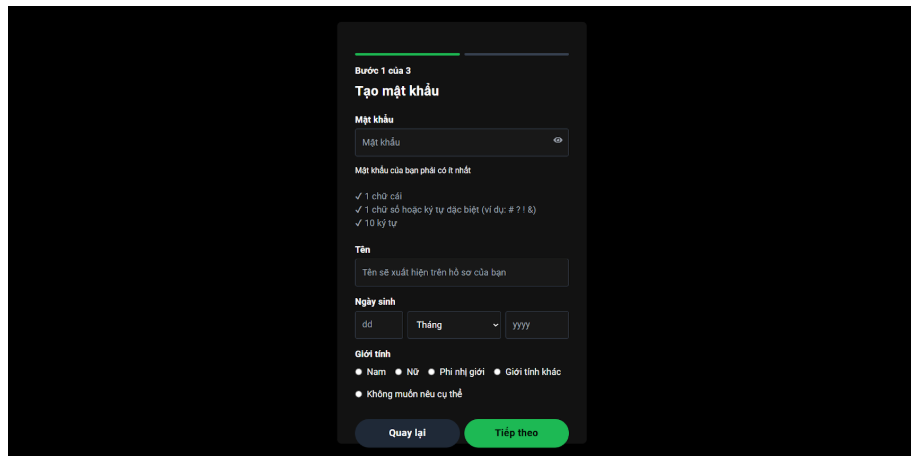
\includegraphics[width=1\linewidth]{images/ui-signup1.png}
    \caption{Giao diện đăng ký}
    \label{fig:ui-signup1.png}
\end{figure}

\begin{figure}
    \centering
    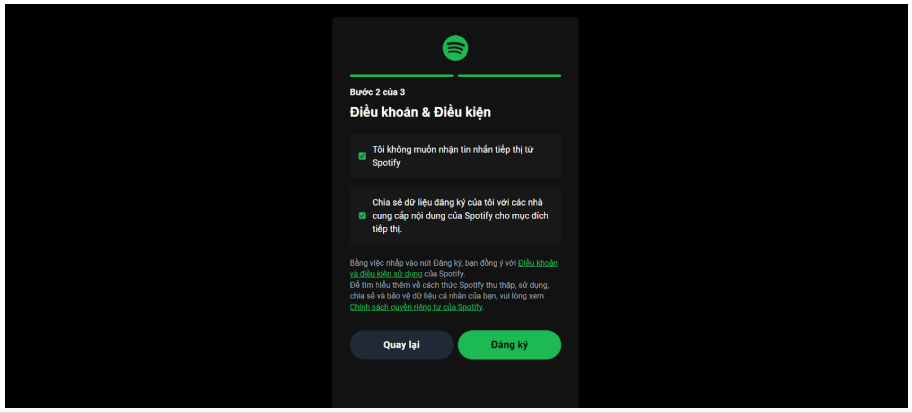
\includegraphics[width=1\linewidth]{images/ui-signup2.png}
    \caption{Giao diện đăng ký}
    \label{fig:ui-signup2.png}
\end{figure}

\begin{figure}
    \centering
    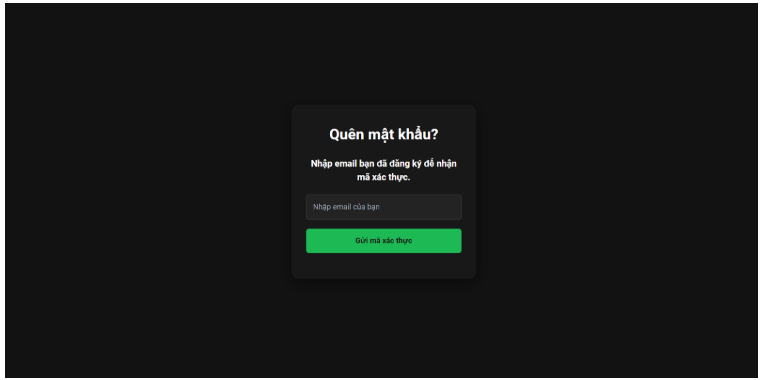
\includegraphics[width=1\linewidth]{images/ui-forgot.png}
    \caption{Giao diện quên mật khẩu}
    \label{fig:ui-forgot}
\end{figure}

\begin{figure}
    \centering
    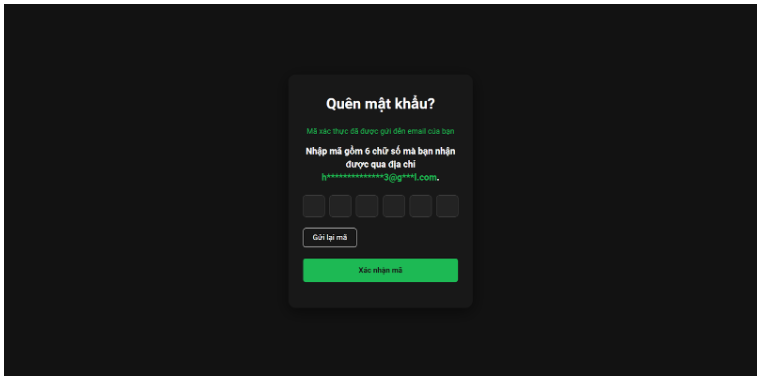
\includegraphics[width=1\linewidth]{images/ui-forgot1.png}
    \caption{Giao diện quên mật khẩu}
    \label{fig:ui-forgot1}
\end{figure}

\begin{figure}
    \centering
    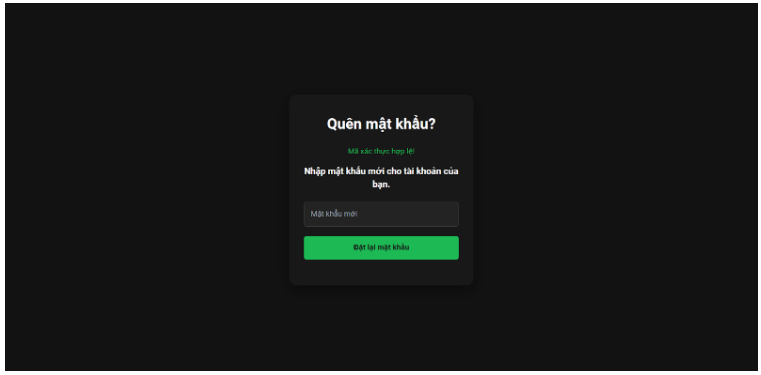
\includegraphics[width=1\linewidth]{images/ui-forgot2.png}
    \caption{Giao diện quên mật khẩu}
    \label{fig:ui-forgot2}
\end{figure}

\begin{figure}
    \centering
    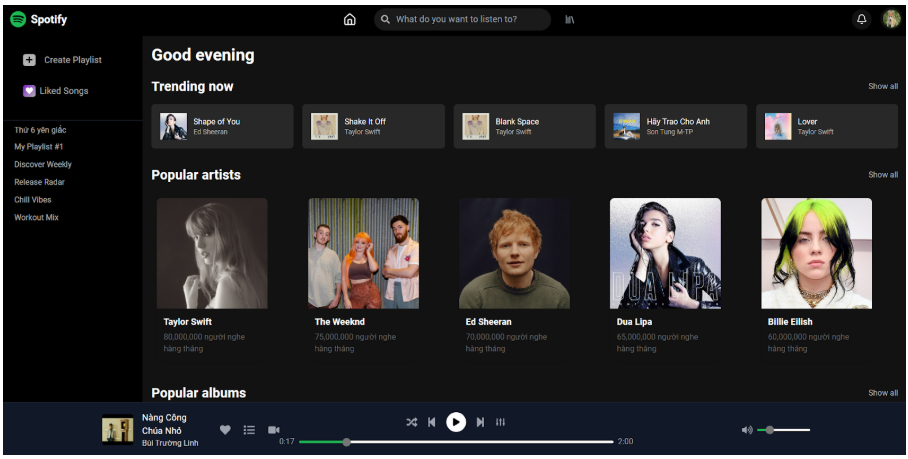
\includegraphics[width=1\linewidth]{images/ui-homepage.png}
    \caption{Giao diện trang chủ}
    \label{fig:ui-homepage}
\end{figure}

\begin{figure}
    \centering
    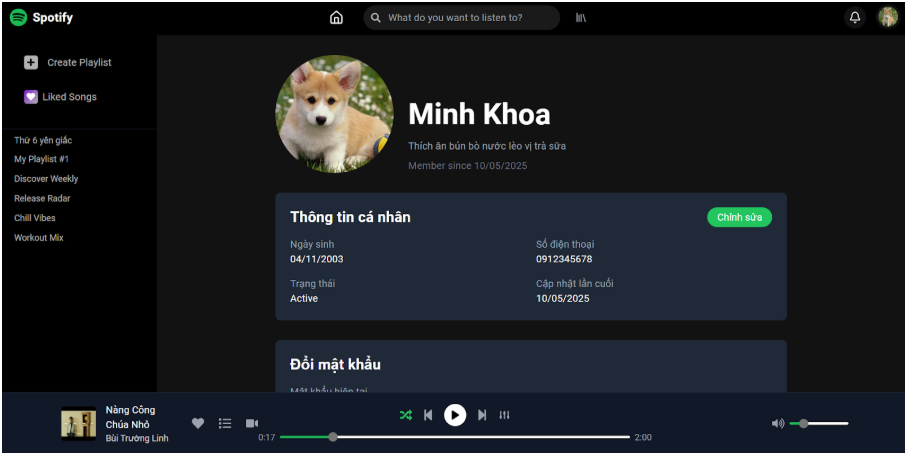
\includegraphics[width=1\linewidth]{images/ui-profile.png}
    \caption{Giao diện hồ sơ}
    \label{fig:ui-profile}
\end{figure}

\begin{figure}
    \centering
    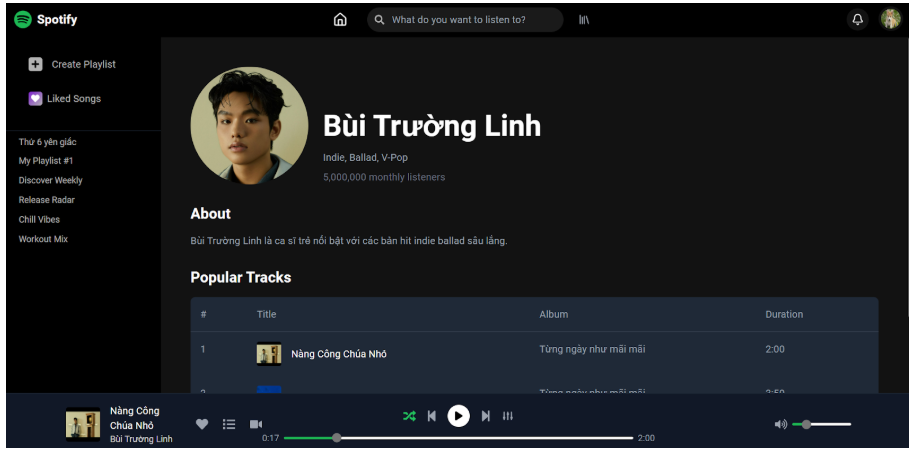
\includegraphics[width=1\linewidth]{images/ui-artist.png}
    \caption{Giao diện nghệ sĩ}
    \label{fig:ui-artist}
\end{figure}

\begin{figure}
    \centering
    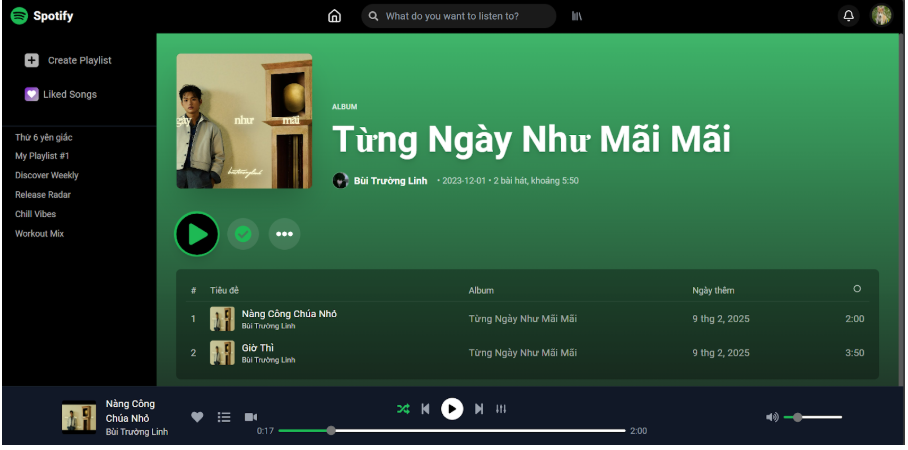
\includegraphics[width=1\linewidth]{images/ui-album.png}
    \caption{Giao diện xem Album}
    \label{fig:ui-album}
\end{figure}

\begin{figure}
    \centering
    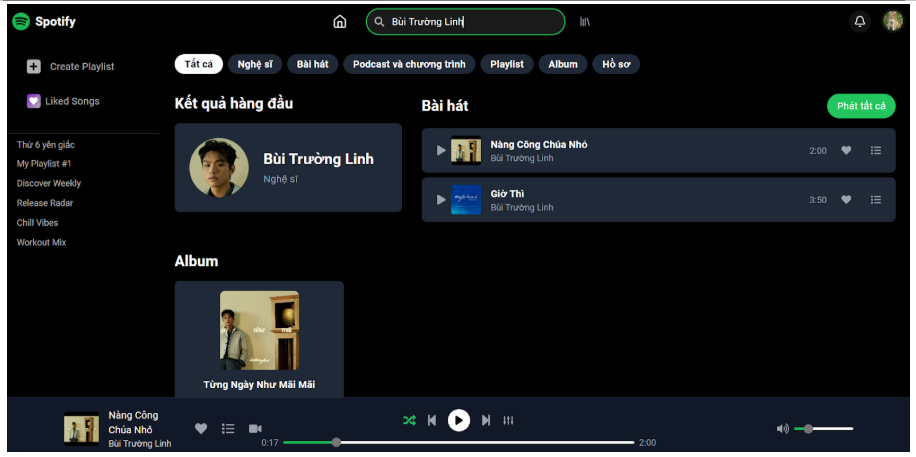
\includegraphics[width=1\linewidth]{images/ui-search.png}
    \caption{Giao diện tìm kiếm}
    \label{fig:ui-search}
\end{figure}

\begin{figure}
    \centering
    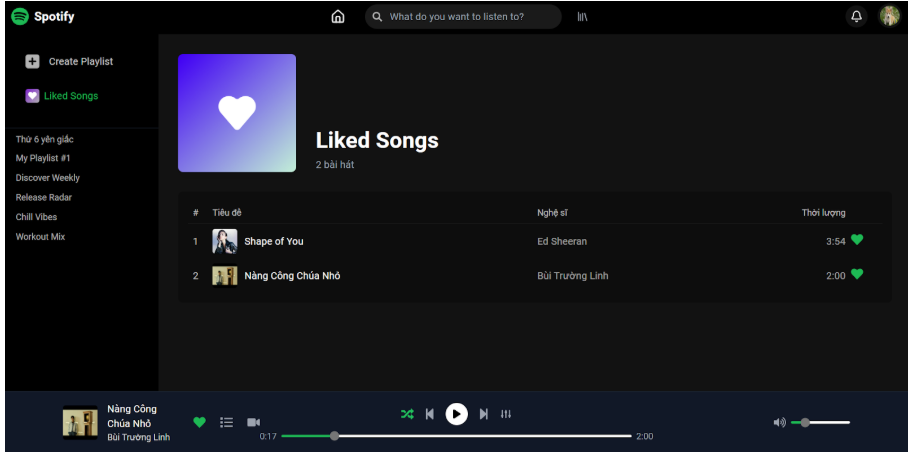
\includegraphics[width=1\linewidth]{images/ui-favorite.png}
    \caption{Giao diện yêu thích}
    \label{fig:ui-favorite}
\end{figure}

\subsection{Trang chủ}
\label{subsec:homepage_ui}
[Chỗ để dán hình ảnh trang chủ]

\subsection{Giao diện phát nhạc}
\label{subsec:music_player_ui}
[Chỗ để dán hình ảnh giao diện phát nhạc]

\subsection{Giao diện phát video âm nhạc}
\label{subsec:video_player_ui}
[Chỗ để dán hình ảnh giao diện phát video âm nhạc]

\subsection{Giao diện tạo album}
\label{subsec:create_album_ui}
[Chỗ để dán hình ảnh giao diện tạo album]

\subsection{Giao diện quản lý bài hát yêu thích}
\label{subsec:favorite_songs_ui}
[Chỗ để dán hình ảnh giao diện quản lý bài hát yêu thích]

\subsection{Trang Admin}
\label{subsec:admin_ui}
[Chỗ để dán hình ảnh trang Admin]

\subsection{Giao diện chat}
\label{subsec:chat_ui}
[Chỗ để dán hình ảnh giao diện chat]

\section{Backend và API}
\label{sec:backend_implementation}

\subsection{API cho chức năng phát nhạc}
\label{subsec:music_api}
[Mô tả ngắn gọn về các API liên quan và có thể có hình ảnh sơ đồ API]

\subsection{API cho chức năng phát video âm nhạc}
\label{subsec:video_api}
[Mô tả ngắn gọn về các API liên quan và có thể có hình ảnh sơ đồ API]

\subsection{API cho chức năng quản lý thư viện người dùng}
\label{subsec:library_api}
[Mô tả ngắn gọn về các API liên quan và có thể có hình ảnh sơ đồ API]

\subsection{API cho trang Admin}
\label{subsec:admin_api}
[Mô tả ngắn gọn về các API liên quan và có thể có hình ảnh sơ đồ API]

\subsection{Giao tiếp gRPC giữa các microservice}
\label{subsec:grpc_communication}
[Mô tả ngắn gọn về cách các microservice giao tiếp qua gRPC và có thể có sơ đồ]